%\documentclass[xcolor=dvipsnames]{beamer}
\documentclass[handout,xcolor=dvipsnames,pdftex,hyperref={colorlinks=false}]{beamer}

% == Packages
\usepackage{xcolor}
\usepackage{graphicx}
\graphicspath{{figures/}}
\usepackage{fancybox}
\usepackage{hyperref}
\usepackage{amsmath,amssymb,amsfonts,bm}
\usepackage{wasysym}
\usepackage{colortbl}
\usepackage[english]{babel}
\usepackage{times}
\usepackage{multirow}
\usepackage{listings}
\usepackage{rotating}
\usepackage{latexsym}
\usepackage{ulem}
\usepackage{tikz}
\usetikzlibrary{positioning,arrows.meta}

\newenvironment{Shaded}{}{}

\usetheme{Warsaw}
\usepackage{helvet}
\definecolor{someblue}{rgb}{0,.1,0.8}
\definecolor{dgreen}{rgb}{0,.6,0.8}
\useoutertheme{infolines}

% == Typesetting helpers
\newcommand\spacingset[1]{\renewcommand{\baselinestretch}{#1}\small\normalsize}
\renewcommand\r{\right}
\renewcommand\l{\left}
\newcommand\makegaps{\addtolength{\itemsep}{.25\baselineskip}}
\newcommand\smallunskip{\vspace{-.25\baselineskip}}
\newcommand\medunskip{\vspace{-.5\baselineskip}}
\newcommand\bigunskip{\vspace{-\baselineskip}}

% == Math / stats
\renewcommand{\epsilon}{\varepsilon}
\newcommand\E{\mathbb{E}}
\newcommand\V{\mathbb{V}}
\newcommand\Y{{\bm Y}}
\newcommand\X{{\bm X}}
\newcommand\D{{\bm D}}
\newcommand\eps{{\bm\varepsilon}}
\newcommand{\Var}{\mathrm{Var}}
\newcommand{\Cov}{\mathrm{Cov}}
\DeclareMathOperator\rank{rank}
\newcommand\indep{\protect\mathpalette{\protect\independenT}{\perp}}
\def\independenT#1#2{\mathrel{\rlap{$#1#2$}\mkern2mu{#1#2}}}

\newcommand{\bs}{\boldsymbol}
\newcommand{\mb}{\mathbf}
% Synth / panel notation -- matched to the tjbal paper conventions
\newcommand{\Ypre}{Y^{\text{pre}}}        % pre-period outcome (scalar or generic)
\newcommand{\Ypost}{Y^{\text{post}}}      % post-period outcome (scalar or generic)
\newcommand{\ypre}{Y^{\text{pre}}_i}      % unit i's pre-period outcome vector
\newcommand{\ypost}{Y^{\text{post}}_i}    % unit i's post-period outcome vector
\newcommand{\Lpre}{\Lambda_{\text{pre}}}  % pre-period factor-loading matrix
\newcommand{\Lpost}{\Lambda_{\text{post}}}% post-period factor-loading matrix
\newcommand{\att}{\tau_{\text{ATT}}}      % ATT estimand
\newcommand{\satt}{\tau_{\text{sATT}}}    % sample ATT
\newcommand{\Tpre}{T_0}                   % last pre-treatment period
\newcommand{\reiv}{r_{\text{eiv}}}        % errors-in-variables residual
\newcommand{\rrec}{r_{\text{rec}}}        % non-recoverability residual
\newcommand{\Wco}{\mb{w}}                 % donor-weight vector
\newcommand{\Gpre}{G^{\text{pre}}}        % pre-period (possibly nonlinear) bridge map
\newcommand{\Gpost}{G^{\text{post}}}      % post-period bridge map

\newtheorem{assumption}{Assumption}

\AtBeginSection[]
{
  \begin{frame}<beamer>
    \frametitle{Outline}
    \tableofcontents[currentsection]
  \end{frame}
}

\title[Synthetic Control]{Synthetic Control}
\subtitle[ ]{PS200C, Spring 2026}
\author[Hazlett]{Chad Hazlett}
\institute[UCLA]{UCLA\\[1ex]\texttt{chazlett@ucla.edu}}
\date{}

\begin{document}

\subject{Talks}

% ============================================================
\begin{frame}
  \titlepage
\end{frame}

\begin{frame}{Roadmap}
\begin{enumerate}\makegaps
  \item Motivation: where DID fails
  \item A DGP we can reason about: the linear factor model
  \item Intuition: balance on $\Ypre$ buys balance on $Y(0)_{\text{post}}$
  \item Prop 99: a first pass
  \item What can go wrong: EIV \& recoverability
  \item Flavors of synth and a bias-decomposition view
  \item Practice and inference
\end{enumerate}
\end{frame}

% ============================================================
\section{Motivation: where DID fails}
% ============================================================

\begin{frame}{Where DID gets uncomfortable}
\textbf{DID (and staggered DID) require no time-varying confounding}, conditional on unit and time FEs.\\[1ex]
That is what ``parallel trends'' encodes.\\[2ex]
\onslide<2-> E.g. In 1989 California's Prop 99 went into effect, raising cigarette taxes. You want to see if it reduced cigarette sales. \\[1ex]
\onslide<3-> What changes over time, is felt differently in different states, and is related to the outcome and treatment chances? E.g.
\begin{itemize}\makegaps
  \item Health consciousness
  \item Anti-tobacco sentiment
  \item Willingness to use tax structure to achieve social aims
\end{itemize}
\end{frame}

\begin{frame}{The hope}
  \small
\textbf{Synthetic control} offers a way to address \emph{time-varying} unobserved confounding by leaning on the \emph{shape} of pre-treatment outcomes to detect the confounding signal.\\[3ex]
\medskip
\onslide<2-> \textbf{Intuition}: If you had a state with same pre-treatment trajectory of cigarette sales ($\ypre$), then it must have similar values on (time-varying) confounders.  Further we can just ``upweight'' states with similar $\ypre$. \\

\bigskip
\onslide<3->  \textbf{This is seductive and popular:} Athey \& Imbens (2017) call it ``arguably the most important innovation in the policy evaluation literature in the last 15 years,'' and the original Abadie--Diamond--Hainmueller (2010) paper has 9k citations.\\

\bigskip
\onslide<4->{... but I've never seen identification assumptions discussed in an  application. When does it actually work? What are the required assumptions?} \\[1ex]

\end{frame}

\begin{frame}{Heads-up: synth is \emph{not} DID}
This should be obvious now but in case you missed it...\\
\begin{itemize}\makegaps
  \item<1-> Synth does \textbf{not} assume parallel trends.
  \item<2-> A common student error is to think of synth as ``a better DID.'' It isn't. It's a different identification strategy.
  \item<3-> In fact, once a synth weighting matches the treated unit at the last pre-treatment period, \emph{DID would just become the diff.}
  %\item<4-> (We'll return to this when we see SDID, which deliberately uses both unit and time weights.)
\end{itemize}
\end{frame}

\begin{frame}{Demystifying: it's mean-balancing}
Most synthetic-control estimators (Abadie's OG, augmented SCM, synthetic DID, \texttt{tjbal} with linear kernel) effectively: \textbf{find donor weights $w$ that make the weighted control's $\Ypre$ match the treated unit's $\Ypre$.}\\[2ex]
\onslide<2->{This is the same cross-sectional weighting/matching you already know --- on the \emph{wide-form} panel where ``X'' is the vector of pre-treatment outcomes $(Y_{i,1}, \ldots, Y_{i,T_0})$.\\[2ex]}
\onslide<3->{What changes between flavors:
\begin{itemize}
  \item what we balance (means? richer features?),
  \item what constraints on $w$ (simplex? entropy? ridge?),
  \item whether we also weight time periods (SDID).
\end{itemize}}
\end{frame}

% ============================================================
\section{A DGP we can reason about}
% ============================================================

\begin{frame}{Pretend we believe the linear factor model}
\[
Y_{it}(0) \;=\; \alpha_i + \lambda_t^\top u_i + \varepsilon_{it}
\]
\small

\begin{itemize}\makegaps
  \item<2-> $u_i \in \mathbb{R}^K$: unit-level \textbf{factor loadings} (time-invariant)
  \item<3-> $\lambda_t \in \mathbb{R}^K$: \textbf{time-varying factors} (common across units)
  \item<4-> $\varepsilon_{it}$: idiosyncratic noise
\end{itemize}
\bigskip
\normalsize
\onslide<5-> This is a vivid DGP you can imagine two ways:\\

\small
\begin{itemize}
\item Unit confounding characteristics ($u_i$) whose impact vary over time ($\lambda_t$).
\item Or time-varying ``signals'' whose influence on unit $i$ depends on ``loadings'' $u_i$.
\end{itemize}
\end{frame}

\begin{frame}{Three latent factors $\lambda_t^{(k)}$ for CA Prop 99}
\begin{center}
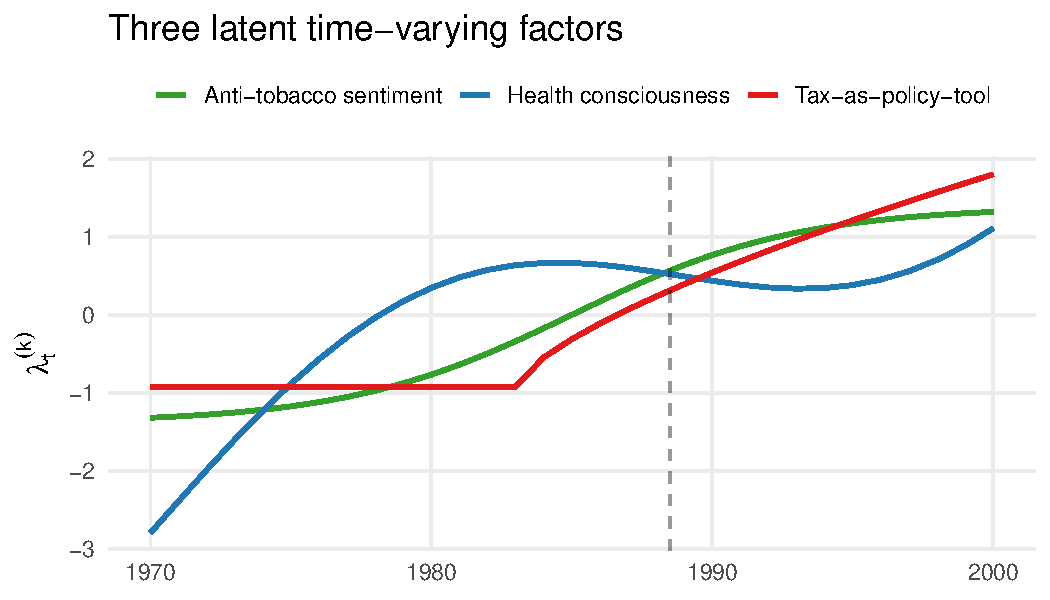
\includegraphics[width=.85\textwidth]{factors.pdf}
\end{center}
Smooth time-varying signals:
health consciousness, anti-tobacco sentiment, tax-as-policy-tool.\\[1ex]
\end{frame}

\begin{frame}{State-level loadings $u_i^{(k)}$}
Imagine state-level loadings ($u_i$) on these such as,
\begin{center}
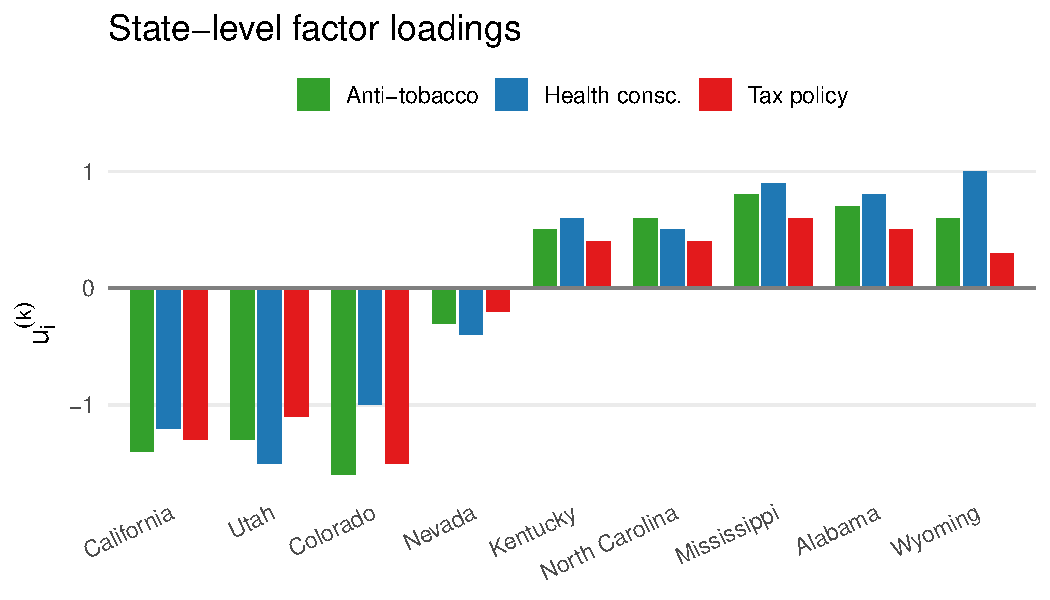
\includegraphics[width=.8\textwidth]{loadings.pdf}
\end{center}
\onslide<2->{CA, UT, CO, NV have high loadings on all three. \\ KY/NC/MS/AL/WY quite different.}
\end{frame}

\begin{frame}{Assembled $Y_{it}(0) = \lambda_t^\top u_i + \varepsilon_{it}$}
\begin{center}
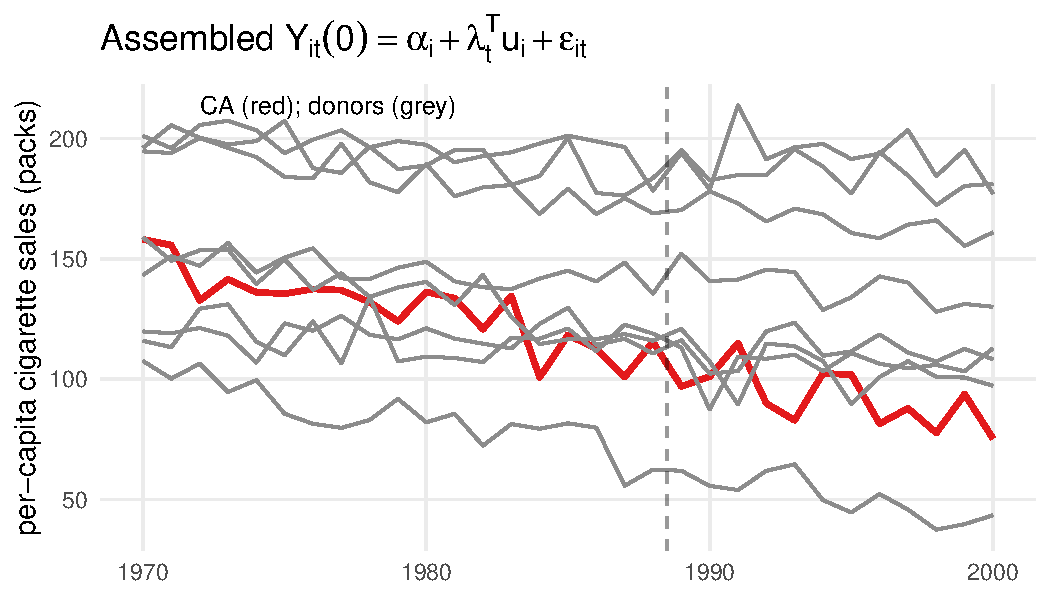
\includegraphics[width=.8\textwidth]{trajectories.pdf}
\end{center}
\onslide<2->{Different states evolve differently --- not because $\lambda_t$ differs, but because their loadings $u_i$ project the same factors differently.}
\end{frame}

\begin{frame}{The estimand and the obstacle}
\textbf{Estimand:} the sample ATT for CA,
\[
\tau_{\text{ATT}} \;=\; \E\!\left[\, Y_{i,T+1}(1) - Y_{i,T+1}(0) \;\middle|\; i = \text{CA} \,\right].
\]
\medskip
\onslide<2->{\textbf{Why DID/FE won't do it:}
\begin{itemize}
  \item $u_i$ is time-invariant --- TWFE can wipe \emph{its mean effect}
  \item but the \emph{differential exposure} $\lambda_t$ is time-varying
  \item TWFE leaves $(\lambda_t - \bar\lambda)^\top u_i$ behind --- exactly the confounder
\end{itemize}}
\bigskip
\onslide<3->{We need to neutralize $u_i$ itself, or at least its post-treatment imprint $\lambda_{T+1}^\top u_i$.}
\end{frame}

\begin{frame}{Connection back to the DID lecture}
We saw at the end of DID:
\begin{quote}
``Ensuring balance on prior outcomes starts to bring you toward other strategies that effectively condition on $\Ypre$, e.g.\ synthetic control.''
\end{quote}
\bigskip
That's the bridge we're crossing today.
\end{frame}

% ============================================================
\section{Intuition for the synth fix}
% ============================================================

\begin{frame}{Intuition: $\Ypre$ encodes $u_i$}
The pre-treatment trajectory of unit $i$:
\[
Y_{i,\text{pre}} \;=\; \Lpre\, u_i + \varepsilon_{i,\text{pre}}, \qquad \Lpre = \begin{bmatrix}\lambda_1^\top \\ \vdots \\ \lambda_T^\top\end{bmatrix}
\]
\onslide<2->{If $\Lpre$ is rich enough, similar $\Ypre$ $\Rightarrow$ similar $u_i$.}\\[2ex]
\onslide<3->{And similar $u_i$ $\Rightarrow$ similar $\lambda_{T+1}^\top u_i$ $=$ similar $Y(0)_{T+1}$.\\[1ex]
That's our identification chain.}
\end{frame}

\begin{frame}{The chain}
So we're hoping: \\
\begin{center}
\textcolor{blue}{balance on $\ypre$ $\rightarrow$ balance on $u_i$ $\rightarrow$ balance on $Y(0)$ $\rightarrow$ sATT}
\end{center}
% \begin{center}
% balance on $\Ypre$ \\[1ex]
% $\Downarrow$ \\[1ex]
% balance on $u_i$ \\[1ex]
% $\Downarrow$ \\[1ex]
% balance on $Y(0)_{T+1}$
% \end{center}
\bigskip
\onslide<2->Plan:  (1) Find donor weights $w$ such that
\small
\[
\sum_{i \in \text{donors}} w_i\, Y_{i,\text{pre}} \;\approx\; Y_{\text{CA},\text{pre}}.
\]
\normalsize
\onslide<3-> (2) Get weights by choosing, with some constraints/penalties:
\small
\[
\widehat{Y(0)}_{\text{CA},T+1} = \sum_i w_i\, Y_{i,T+1}
\]
\normalsize
\onslide<4-> (3) Then estimate sATT with:
\small
\[ \widehat{\tau} = Y_{\text{CA},T+1} - \widehat{Y(0)}_{\text{CA},T+1}\]
\end{frame}

% \begin{frame}{``DID just becomes the diff''}
% If $\sum w_i Y_{i,T} \approx Y_{\text{CA},T}$, then the DID estimator
% \[
% (Y_{\text{CA},T+1} - Y_{\text{CA},T}) - \sum_i w_i (Y_{i,T+1} - Y_{i,T})
% \]
% \medskip
% collapses to
% \[
% Y_{\text{CA},T+1} - \sum_i w_i\, Y_{i,T+1}
% \]
% \bigskip
% because the pre-period terms cancel.\\[1ex]
% \onslide<2->{Synth and SDID differ in whether you also weight \emph{time periods} and what feature you balance on --- not in spirit.}
% \end{frame}

% \begin{frame}{Abadie's classic SCM, demystified}
% Abadie--Diamond--Hainmueller (2010):
% \[
% \min_{w \in \Delta} \;\bigl\lVert\, Y_{\text{CA},\text{pre}} - \sum_i w_i\, Y_{i,\text{pre}} \,\bigr\rVert^2_V
% \]
% with $w \geq 0,\ \sum w_i = 1$, and a covariate matrix $V$ that can include extras (beer, income, age 15--24, retail price).\\[2ex]
% \onslide<2->{Strip away the simplex constraint and $V$, and this is just\\
% \emph{mean balancing on $\Ypre$} --- the same as ebal / kbal-linear / weighted ATT.}\\[2ex]
% \onslide<3->{The simplex matters in practice (interpolation, sparse weights), but does not change the identification logic.}
% \end{frame}

\begin{frame}{Sanity check: which donors get picked?}
Toy LFM, 8 donors (UT, CO, NV + KY, NC, MS, AL, WY). Solve for simplex weights $\Wco$ matching CA's $\ypre$:
\begin{center}
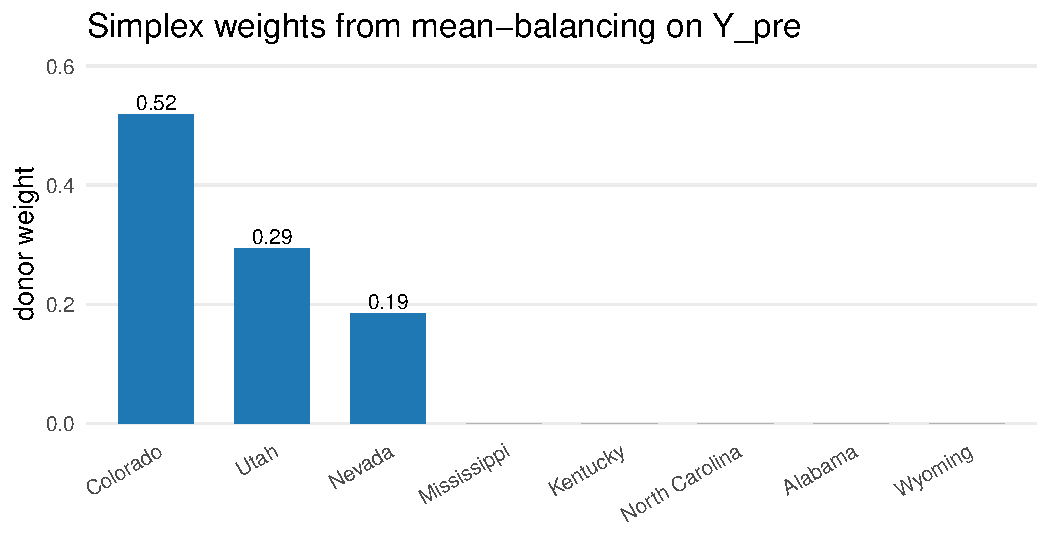
\includegraphics[width=.78\textwidth]{weights.pdf}
\end{center}
\end{frame}

\begin{frame}{Does it balance on confounding characteristics ($u$)?}
\begin{center}
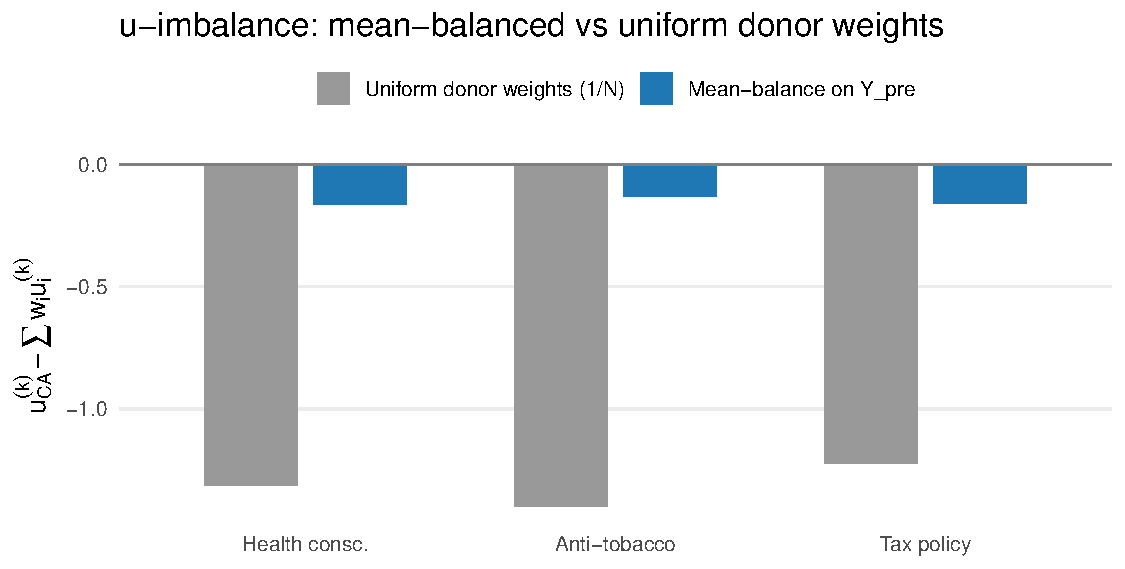
\includegraphics[width=.75\textwidth]{balance_compare.pdf}
\end{center}
\small
\textbf{Implied bias on $Y(0)_{T+1}$}: 
\begin{itemize}
\item Uniform weights: $\text{bias}=\text{imbal}(u_i)^{\top}\lambda_{T+1} \approx \textbf{19}$ packs/capita
\item Mean-balance: $\text{bias}=\text{imbal}(u_i)^{\top}\lambda_{T+1} \approx \textbf{0.7}$ packs/capita
\end{itemize}
\end{frame}

% ============================================================
\section{Prop 99: Let's try it for real.}
% ============================================================

\begin{frame}{California Proposition 99, real data now}
\begin{center}
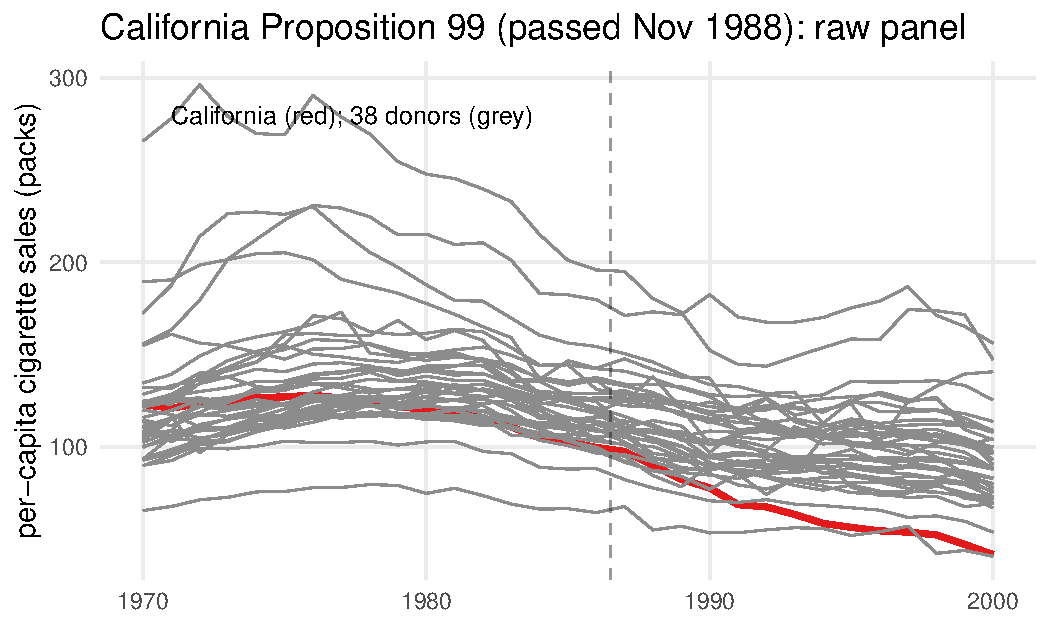
\includegraphics[width=.7\textwidth]{prop99_panel.pdf}
\end{center}
\small
\begin{itemize}
\item Per-capita cig. sales, 1970--2000, CA (red) vs.\ 38 donor states (grey).
\item I use \textbf{1987 as the first treated period}. ADH used 1989.\footnote{\scriptsize 1987: Proposal made; coalition formed, initiative drafted; 1.1M signatures gathered late-1987 through May 1988; ballot passed Nov 1988; tax effective Jan 1989. So: anticipatory purchasing plausible in 1987-1988.}
\end{itemize}
\end{frame}

\begin{frame}[fragile]{The tool: \texttt{tjbal}, linear kernel = mean balancing}
\begin{small}
\begin{verbatim}
library(tjbal)
fit_lin <- tjbal(
  data   = df,
  Y      = "cigsale",
  D      = "D",
  index  = c("state", "year"),
  demean = FALSE,
  kernel = FALSE   # FALSE = linear = mean balance on Y_pre
)
\end{verbatim}
\end{small}
\medskip
That's the whole call. We'll flip \texttt{kernel = TRUE} later.
\end{frame}

\begin{frame}{Synthetic California (linear kernel)}
\begin{center}
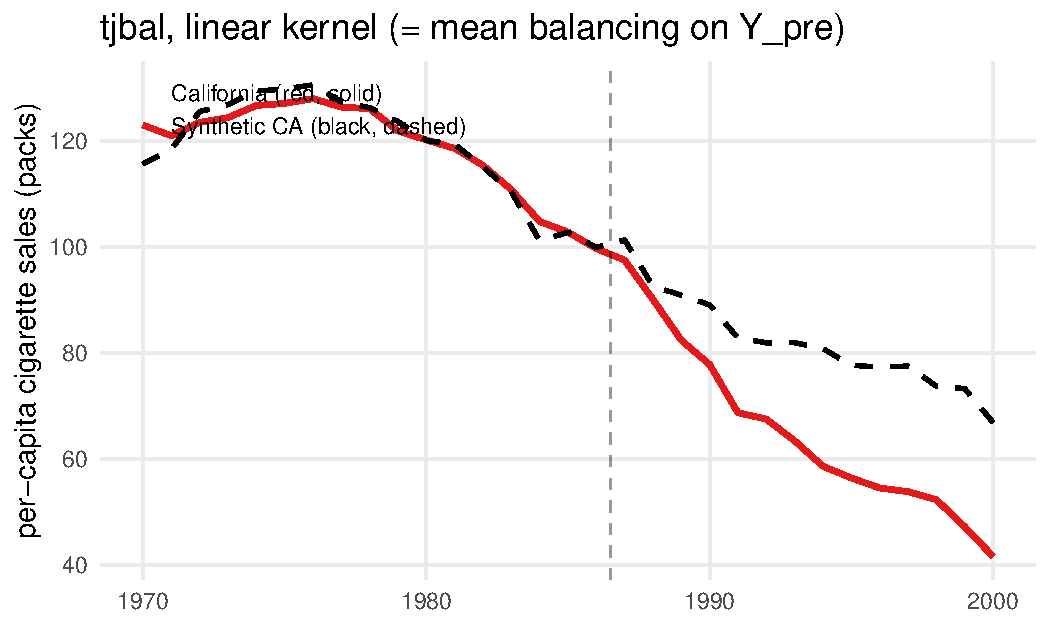
\includegraphics[width=.9\textwidth]{prop99_linear_fit.pdf}
\end{center}
\small
\onslide<2->{Pre-period fit looks good. Post-period gap: CA falls below the synthetic.}
\end{frame}

\begin{frame}{Estimated effect (linear kernel)}
\begin{center}
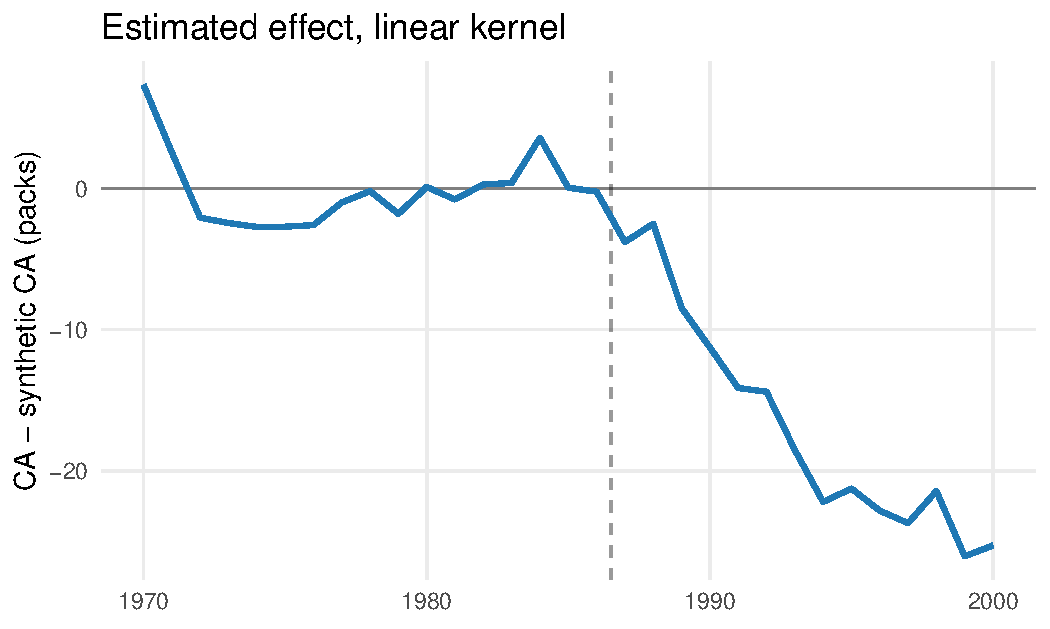
\includegraphics[width=.9\textwidth]{prop99_linear_gap.pdf}
\end{center}
\footnotesize
\onslide<2->{Average post-tx ATT $\approx -17$ packs per capita per year (1987 onward).\\
(Original SCM gives $\approx -19$)}
\end{frame}

% \begin{frame}{Pause: Should we believe it?}
% We balanced on $\Ypre$, and in an LFM we saw how that can improve balance on $u_i$.\\[2ex]
% \onslide<2->{\textbf{Is that enough?}\\[1ex]}
% \onslide<3-> Even if DGP does follow the LFM, two main things to worry about:\\[1ex]
% \onslide<4->{
% \begin{enumerate}
%   \small
%   \item Errors in variables (EIV) --- a finite-sample / noise issue (reason we didn't get exact balance)
%   \item Recoverability --- an \emph{identification} issue
% \end{enumerate}}
% \end{frame}

% ============================================================
\section{What can go wrong}
% ============================================================

% \begin{frame}{Reframe: you are conditioning on $\Ypre$}
%   \small
% What we've done is, mechnically, conditioning on $\ypre$.\\[2ex]
% \bigskip
% That would be great if we believed \textbf{sequential ignorability}:
% \[
% Y(0)_{\text{post}} \;\indep\; D \;\;\big|\;\; \Ypre.
% \]
% \onslide<2->\textbf{But we don't;} the confounders we need are $u_i$; $\ypre$ is a noisy proxy per
% \[
% \Ypre = \underbrace{\Lpre u_i}_{\text{signal}} + \underbrace{\varepsilon_{i,\text{pre}}}_{\text{noise}}.
% \]
% \onslide<3->{Conditioning on a noisy proxy $\neq$ conditioning on the latent.}
% \end{frame}

\begin{frame}{Worry 1: EIV bias}
  \small
Two main problems here. The first is \textbf{errors in variables} (EIV):
Balancing on a noisy version of $u_i$ leaves residual imbalance in the true $u_i$.\\[2ex]
\onslide<2->{\textbf{Bias}: scales with $\sigma_\varepsilon$ relative to signal.}\\[2ex]
\onslide<3->{\textbf{Shrinks with $T$}: more pre-periods = better-resolved $u_i$ (per-state averages of $\varepsilon$ shrink as $1/\sqrt{T}$).}\\[2ex]
\onslide<4->{This is a \emph{finite-sample} problem. Data fixes it eventually.\\[2ex]
The next problem is not so kind.}
\end{frame}

\begin{frame}{Worry 2: Recoverability}
\small
Pretend there is no noise,  $\ypre = \Lpre u_i$\\[2ex]

\onslide<2-> When does balance on $\Lpre u_i$ buy you balance on $u_i$? \\[2ex]

\onslide<3-> Formally: $\lambda_{T+1}$ must lie in the row span of $\Lpre$ --- a \textbf{rank condition} required on top of the LFM. \\[2ex]

\onslide<4-> {In plain English: every confounder that affects post-treatment outcomes must leave a footprint in $\ypre$ that's \emph{distinguishable} from other confounders' footprints.\footnote{ \scriptsize The rank condition, LPO
  (post-outcome is a linear function of $\ypre$ with the same coefficients across units), and the ``distinguishable footprints'' idea are three views of the same condition, with the same failure modes. See Appendix for a trip down the rabbit hole.}}\\[2ex]

\onslide<5-> This is an \textbf{identification-level} assumption, not a simple regularity condition. More $N$ helps estimation, but doesn't fix it.
\end{frame}

\begin{frame}{Concretely, what breaks recoverability?}
  \small
  As usual, the counterexamples help us see clearly.\\
  \bigskip
\textbf{Counter 1: Pre-period too short to disentangle the confounders.}
\footnotesize With $K$ confounders but only $T_{\text{pre}} < K$ pre-periods, distinct confounders leave indistinguishable footprints --- $\ypre$ literally can't tell them apart.\\[2ex]
\small
\onslide<2-> \textbf{Counter 2: Imbalanced sleeping giants.}
\footnotesize
A confounder with little variation before treatment, more after, AND whose $u_i$ is imbalanced across treatment arms. The pre-period leaves \emph{no} footprint for it at all --- it's silent. Then it wakes up at $T+1$.\\
I.e.\ something newly changing in 1987 onward, felt more by CA.

\begin{center}
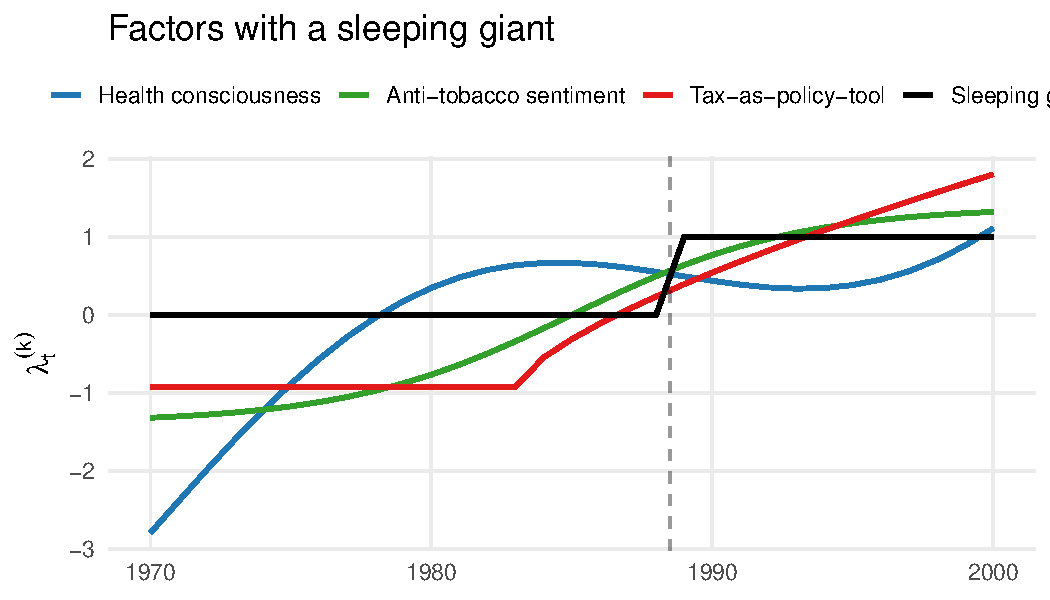
\includegraphics[width=.5\textwidth]{factors_with_sg.pdf}
\end{center}
\end{frame}

\begin{frame}{Insufficient periods demo: 3 factors, only 2 pre-periods}
\small
Keep the same 3-factor LFM, but balance only on $\ypre$ from \emph{1985 and 1986} (so $T_{\text{pre}}=2 < K = 3$). The simplex weights perfectly match those two years --- but the rank condition fails, so balance on $u_i$ does not follow:
\begin{center}
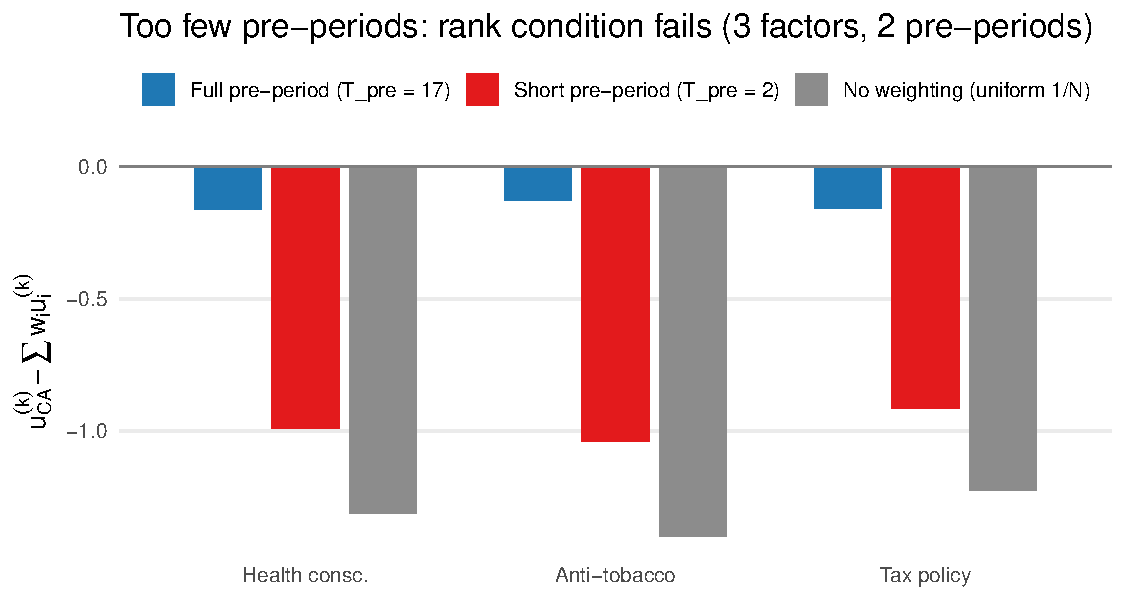
\includegraphics[width=.75\textwidth]{balance_short_T.pdf}
\end{center}
%\onslide<2-> Imbalance on each $u_i^{(k)}$ jumps from $\sim 0.2$ (full $T_{\text{pre}}=17$, blue) to $\sim 1.0$ (short $T_{\text{pre}}=2$, red) --- as bad as if we hadn't balanced at all.
\end{frame}

% \begin{frame}{Sleeping giants: what it does}
% \begin{center}
% 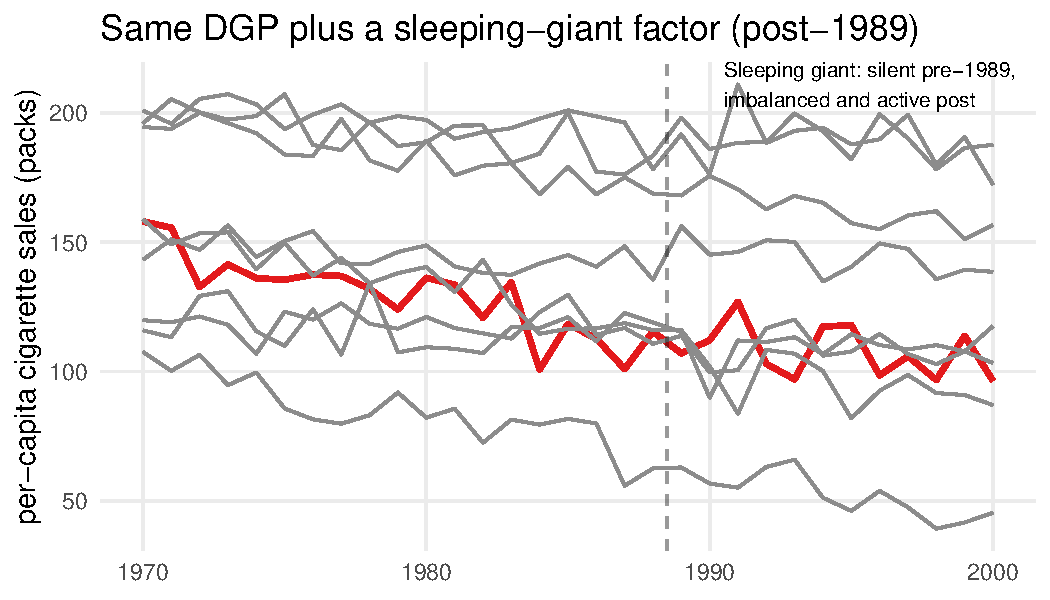
\includegraphics[width=.8\textwidth]{sleeping_giant.pdf}
% \end{center}
% \small
% \onslide<2-> \textbf{Pre-period}: doesn't know; trajectories untouched, still perfect balance.\\
% \textbf{Post-period}: new factor pushes $Y(0)$ in CA, not in synthetic counterfactual.\\[1ex]
% \end{frame}

\begin{frame}{Sleeping giant demo: Uh oh!}
\small
\begin{itemize}
\item Pre-treatment period is uninformative about $u^{(4)}$
\item  Suppose the 4th factor has $u_{\text{CA}}^{(4)} = 1$ while donors have $u_i \sim \mathrm{Unif}(-0.5, 0.5)$.
\end{itemize}
\begin{center}
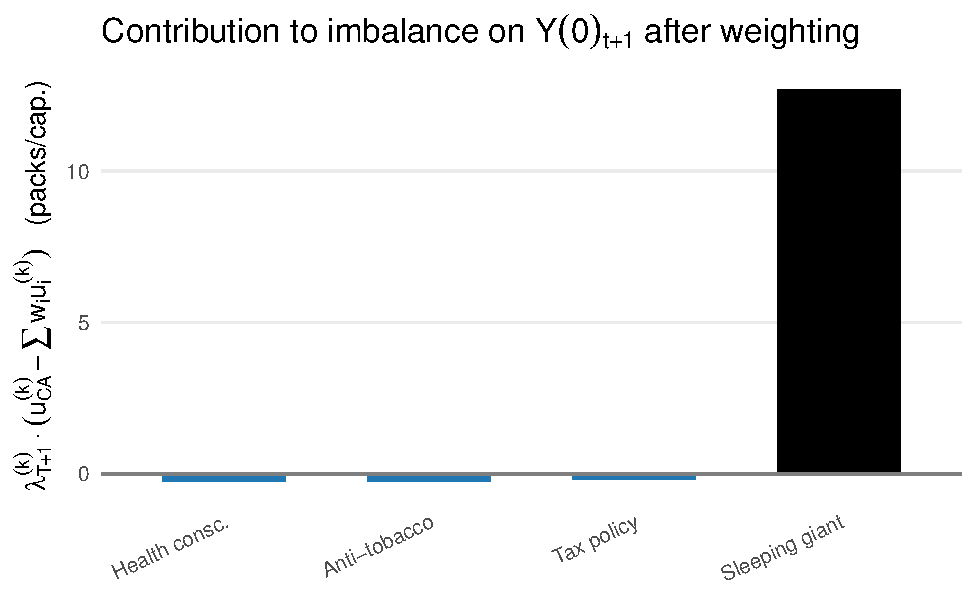
\includegraphics[width=.6\textwidth]{balance_check.pdf}
\end{center}
%\onslide<2->{Same weights $\Wco$ as before --- $\ypre$ didn't change.\\
%Visible-factor bias contributions still tiny (sum $\approx -0.2$).\\
%Sleeping-giant bias: $\lambda_{T+1}^{(4)} \cdot (u_{\text{CA}}^{(4)} - \sum w_i u_i^{(4)}) \approx 10 \cdot 1.33 \approx \textbf{13 packs/capita}$ at $T{+}1$.\\[0.5ex]
%That's about half of Abadie's measured Prop-99 effect, from \emph{one} silent factor.}
Any factor that's invisible in the pre-period leaves no trace to balance on...effectively unobserved confounding.
\end{frame}

% \begin{frame}{Why recoverability matters more than EIV}
% \begin{itemize}\makegaps
%   \item<1-> EIV: noisy proxy. Bias shrinks with more pre-periods. \textbf{Finite-sample.}
%   \item<2-> Recoverability: the proxy doesn't \emph{point at} the right thing. Bias persists. \textbf{Identification.}
%   \item<3-> The sleeping giant is the cartoon, but the issue is general: any factor that's invisible in the pre-period leaves no trace to balance against.
% \end{itemize}
% \bigskip
% \onslide<4->{This is the synth analogue of unmeasured confounding under SOO --- and like there, the cure is substantive knowledge of the DGP, not more data.}
% \end{frame}

% \begin{frame}{Why mean balance --- and the weaker hope: LPO}
% We've been balancing the \emph{mean} of $\Ypre$ across donors. When does that suffice?\\[1ex]
% \onslide<2->{\textbf{Linearity in Prior Outcomes (LPO):}
% \[
% Y_{i,T+1}(0) \;=\; \alpha + \beta^\top \ypre + \eta_i, \qquad \E[\eta_i \mid D_i] = 0.
% \]
% A weaker hope than full LFM: just \emph{linear in the pre-trajectory}.}\\[1ex]

% \onslide<3->{Under LPO, weights $\Wco$ with $\sum_i w_i \ypre = Y^{\text{pre}}_{\text{CA}}$ give
% \[
% \sum_i w_i\, Y_{i,T+1}(0) \;=\; \alpha + \beta^\top Y^{\text{pre}}_{\text{CA}} + \sum_i w_i\, \eta_i
% \;\approx\; Y_{\text{CA},T+1}(0).
% \]}
% \onslide<4->{When LPO fails: need to balance \emph{richer features} of $\ypre$ (kernel balancing).\\
% But the sleeping-giant problem persists --- no features of $\ypre$ recover a silent-pre factor.}
% \end{frame}

\begin{frame}{Aside: lagged-DV regression does the same thing}
\textbf{LDV regression:}
\[
Y_{i,T+1} \;=\; \alpha + \beta^\top \ypre + \tau D_i + \varepsilon_i.
\]
\onslide<2->By FWL, $\hat\tau = \Cov(Y_{i,T+1}^{\perp \ypre},D_i^{\perp \ypre})/\Var(D_i^{\perp \ypre})$.\\[1.5ex]

\onslide<3->...i.e. anything linear in $\ypre$ is removed, just as mean balancing on $\ypre$ removes anything linear in it from ATT.\\ %{\textbf{Does the same work as mean-balancing synth:} anything linear in $\ypre$ is taken care of either way.}\\[1.5ex]
\bigskip
\onslide<4->{\textbf{Where they differ:} the \emph{nature of the implied weights}.
\begin{itemize}\makegaps
  \footnotesize
  \item synth: sparse, $w_i \geq 0$, $\sum w_i = 1$ --- may fail to find balance to varying degrees, but refuses extrapolation.
  \item LDV (OLS): never visibly fails, but the equivalent weights can be negative, indicating extrapolation gambles.\footnote{\footnotesize Crazy but true: with exactly one treated unit, the LDV gives you same answer as imputing/g-comp that trains on controls only, predicts on treated and contrasts with observed treated outcome. Does not hold with more treated units.}
\end{itemize}}

\end{frame}

\begin{frame}{Back to Prop 99: LDV $\approx$ mean-balancing synth}
Fit this and plot $\hat{\tau}_{t^*}$ in each post-period,\footnote{ \footnotesize For pre-period $t^*$, drop $t^*$ from the regressors (leave-one-out placebo).}
\[
Y_{i,t^*} \;=\; \alpha + \beta^\top Y_{i,1970:1986} + \tau_{t^*}\,D_i + \varepsilon_i,
\]
\begin{center}
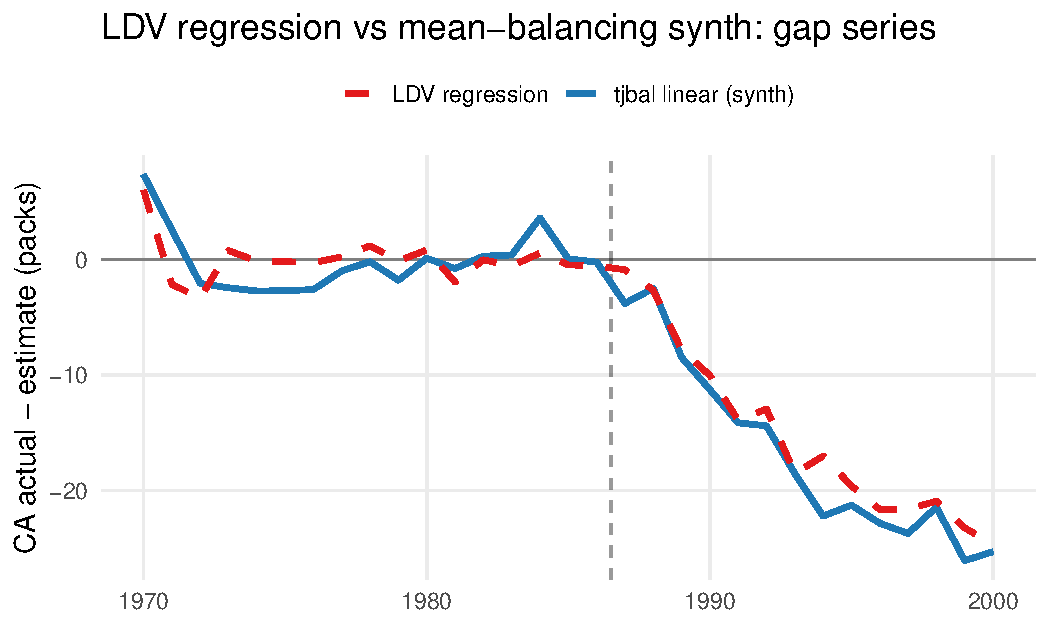
\includegraphics[width=.65\textwidth]{prop99_ldv_vs_tjbal.pdf}
\end{center}
% \onslide<2-> Average post-treatment: \textbf{LDV} $\approx -15.4$, \textbf{tjbal-linear} $\approx -16.9$ packs/capita.\\
% \onslide<3-> Same identifying content (linear in $\ypre$); the small difference is OLS-vs-simplex weighting, and OLS can extrapolate outside the donor hull.
\end{frame}

% ============================================================
\section{Flavors and bias decomposition}
% ============================================================

% \begin{frame}{Two buckets of bias (the tjbal view)}
% For \emph{any} synth-class estimator, the bias splits into:
% \bigskip
% \begin{center}
% \begin{tabular}{p{0.42\textwidth}|p{0.42\textwidth}}
% \textbf{Shrinks with data} & \textbf{Identification} \\
% \hline
% balancing optimization error\newline
% $\downarrow$ as $n \to \infty$ &
% non-recoverability ($r_{\text{rec}}$)\newline
% \emph{does not shrink} \\
% \\
% EIV ($r_{\text{eiv}}$)\newline
% $\downarrow$ as $T \to \infty$ &
% needs a \emph{No Imbalanced Sleeping Giants}--style assumption
% \end{tabular}
% \end{center}
% \bigskip
% \onslide<2->{\textbf{Key:} more data $\neq$ identification. The sleeping giant is structural.}
% \end{frame}

\begin{frame}{The family of synth estimators}
  \small
All are weighted-control estimators differing in what they balance:
\smallskip
\begin{itemize}\makegaps
  \item<1-> \textbf{Classical SCM (Abadie):} mean-balance $\Ypre$ (and optional covariates) on the simplex
  \item<2-> \textbf{Augmented SCM (Ben-Michael et al.):} SCM + outcome-model bias correction
  \item<3-> \textbf{Synthetic DID (Arkhangelsky et al.):} unit weights to balance ``who,'' time-weights to anchor a DID-on-synth step; ridge regularization
  \item<4-> \textbf{tjbal (Hazlett, Xu):} balance kernel features of $\Ypre$; captures slope/curvature, scale-invariant
  \item<5-> ... and many others.
\end{itemize}
\bigskip
\onslide<5->{While some of these add in fallback, the core identification concerns are relevant to all.}
\end{frame}

\begin{frame}{Prop 99 across four estimators}
\begin{center}
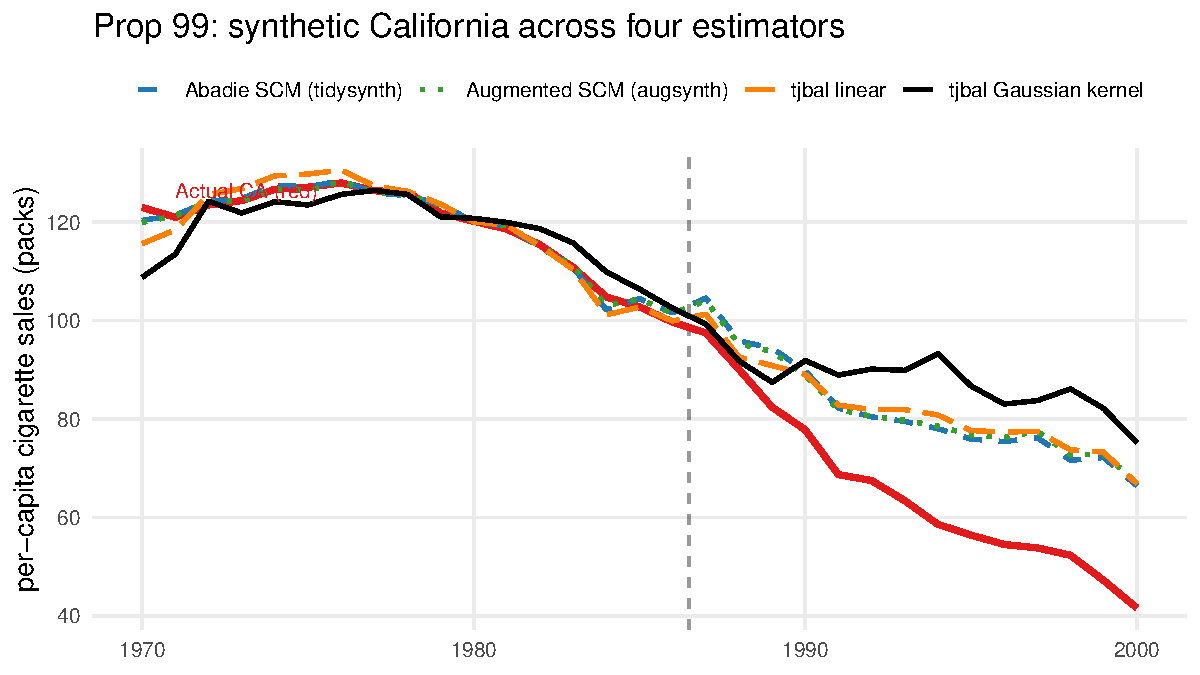
\includegraphics[width=.8\textwidth]{prop99_synth_comparison.pdf}
\end{center}
\small
\onslide<2-> Post-treatment average ATT (1987 onward):
\footnotesize
\begin{itemize}\smallunskip
\item Abadie SCM (tidysynth): $\approx -16.5$
\item Augmented SCM (augsynth): $\approx -16.7$
\item tjbal linear: $\approx -16.9$
\item tjbal Gaussian kernel: $\approx -22.7$
\end{itemize}
%\onslide<3-> The three linear-flavored estimators cluster tightly; flipping to a Gaussian kernel (richer features of $\ypre$) shifts the estimate. Identification requirements unchanged.
\end{frame}

\begin{frame}{Broader view: Bias decomposition under general setting}
\small
Instead of imposing a DGP, doing mean balancing, and asking if it ``is identified,'' consider the weakest setting and broader class of balancing estimators and just look at bias terms.\footnote{Following the \texttt{tjbal} manuscript (Asher, Hazlett, Xu, in progress); active area of research.}
\begin{itemize}\makegaps
\item Assume only latent ignorability: $Y_i(0) \indep D_i \mid u_i$
\item And weakest compatible DGP: $Y_i(0) = g(u_i) + \epsilon_i$.
\item And that you balance on \textit{some} (possibly nonlinear) features $\phi(\ypre)$.
\end{itemize}
\end{frame}

\begin{frame}{Broader view: Bias decomposition under general setting}
\onslide<1-> Under this, the bias of the synth-type estimator decomposes as:
\[
\widehat\tau - \tau \;\approx\; \underbrace{r_{\text{bal}}}_{\text{balancing}} \;+\; \underbrace{\reiv}_{\text{EIV}} \;+\; \underbrace{\rrec}_{\text{recoverability}} \;+\; \underbrace{\epsilon_{T+1}}_{\text{post-noise}}
\]
\small
\onslide<2->
\begin{description}\smallunskip
\item[$r_{\text{bal}}$] How well your weights actually achieve balance on the chosen features. Shrinks with $N$ and a good optimizer.
\item[$\reiv$] $\ypre$ is a noisy view of $u_i$. Shrinks as $T_{\text{pre}} \to \infty$, but worry-worthy in finite $T$.
\item[$\rrec$] Confounding not captured by $\phi(\ypre)$, i.e. bias due to sleeping giants \textbf{does not shrink with data}.
\item[$\epsilon_{T+1}$] Mean-zero; doesn't bias but adds variance (scales with $\|\hat w\|^2$).
\end{description}
\small
\onslide<3-> Tradeoffs:  choice of $\phi$ may help ensure $\rrec$ isn't due to specification in short $T$, but can worsen $r_{\text{bal}}$ and $\reiv$. 
\end{frame}

% ============================================================
\section{Practice and inference}
% ============================================================

\begin{frame}{Practical considerations:}

\begin{itemize} \makegaps
  \small
\item<1-> Taking care with the pre-treatment window:  You want more $T$, but emphasize time when the relevant confounders are \emph{awake} (so, usually more recent).

\item<2-> \textbf{Treatment-year coding.} Watch out for anticipation, as relevant in the Prop 99 case.

\item<3-> \textbf{Multiple treated units, staggered adoption.} Fine, with care to use correct donor pool at each wave. (e.g. \texttt{tjbal} handles automatically)

\item<4->  \textbf{Pre-fit quality}: how well does $\sum w_i Y_{i,\text{pre}}$ track $Y_{\text{CA},\text{pre}}$? Failure here is failure to even condition on $\ypre$.

\item<5-> \textbf{Placebo-in-time}: shrink the pre-window, ``predict'' the held-out periods. Detects recoverability problems within the pre-period.

\item<6-> \textbf{Placebo-in-space}: re-estimate with each donor as ``treated.'' Tells you the spread of placebo effects. Can especially check on ``units most likely to have been treated'' per some propensity score model.

\item<7-> \textbf{Weight inspection}: For sanity check, interpretation, and because extreme weights (high concentration) are brittle.
\end{itemize}
\end{frame}

% \begin{frame}{Diagnostics}
% \begin{itemize}\makegaps

% \end{itemize}
% \bigskip
% \onslide<5->{None of these prove identification. They falsify badly-supported claims.}
% \end{frame}

\begin{frame}{Inference (briefly)}
 \begin{itemize}\makegaps
   \item<1-> \textbf{One treated unit}: genuinely hard. No nice CLT. Permutation/placebo plots are the default. But could simply use LDV.
   \item<2-> \textbf{$\geq 2$ treated units}: jackknife works (the tjbal default).
  %  \item<3-> Bootstrapping requires care --- the weights depend on the donor pool, so naive resampling breaks.
 \end{itemize}
\bigskip
 \onslide<3->{The honest summary: in synth, the point estimate is usually the work, and inference is a sanity check rather than a guarantee.}
 \end{frame}

\begin{frame}{Wrap-up}
\textbf{Synthetic control is not a panacea, of course.}\\[1ex]
\begin{itemize}\makegaps
\item<2-> It does avoid parallel trends / no time-varying confounders. YAY!
\item<3-> Instead hopes for \textit{recoverability}: $\ypre$ encodes sufficient evidence for the ``types'' of units ($u_i$) so that conditioning on $\ypre$ is as good as conditioning on $u_i$.
\begin{itemize}
\item Enough periods, no (imbalanced) sleeping giants.
\end{itemize}
\item<4-> On top of this, estimation grapples with: 
\begin{itemize}
\item EIV bias
\item  What notion of similarity in $\ypre$ encodes similarity in $u$.
\end{itemize}
\end{itemize}
\end{frame}

\begin{frame}{Wrap-up continued}
\onslide<1-> Where does that leave you?\\
\footnotesize
\begin{itemize}\makegaps
\item<1-> More periods is good. Imbalance on $\ypre$ after weighting is pretty bad.
\item<2-> Try mean balance first, then consider higher order if you can afford it. 
\item<3-> Be humble, as usual...as ever, the procedure doesn't make the result causal.
\end{itemize}
\normalsize
\medskip
\onslide<2-> Some reasons for hope (speculative):\\
\footnotesize
\begin{enumerate}
\item<3-> If you get decent mean balance on $\ypre$ then you are getting DID for free (or use sDID etc.), but you are at least adding balance on whatever is linear in $\phi(\ypre)$.
\item<4-> You might be able to argue that time-varying confounders are \textit{smooth} and so cannot be sharp sleeping giants. 
\begin{itemize} 
  \footnotesize
  \item Use domain expertise: why the treated units took treatment when they did, and what realistically influences $Y_t$ at scale...can help rule out the ``suddenness'' of a sleeping giant.
\end{itemize}
\item<5-> Placebos tests can help ensure you are at least catching the structure that exists prior to treatment, leaving you with genuine sleeping giants to worry about. 
\end{enumerate}
\end{frame}

% \begin{frame}{Summary}
% \begin{itemize}\makegaps
%   \item Synth $=$ weighted-control estimator, mean-balancing on $\Ypre$ in the classical case
%   \item LFM is the right DGP to teach with: $Y_{it}(0) = \lambda_t^\top u_i + \varepsilon_{it}$
%   \item Identification chain: balance $\Ypre$ $\Rightarrow$ balance $u_i$ $\Rightarrow$ balance $Y(0)_{\text{post}}$
%   \item Two failure modes: EIV (shrinks with $T$) and recoverability (sleeping giants; does not shrink)
%   \item Flavors differ in features balanced and constraints on $w$ --- the identification story is the same
%   \item Inference: jackknife if $\geq 2$ treated; placebos otherwise
% \end{itemize}
% \end{frame}

% ============================================================
\appendix
\section*{Appendix: rank condition $=$ LPO}
% ============================================================

\begin{frame}{Appendix: rank condition $=$ LPO}
\small
\onslide<2-> We have three views to tie together:
\begin{itemize}
  \item Formal: $\lambda_{T+1}$ lies in the row span of $\Lpre$.
  \item LPO: $Y_{i,T+1}(0)$ is a linear function of $\ypre$ --- same coefficients for every unit.
  \item Footprints: every confounder leaves a distinguishable trace in $\ypre$.
\end{itemize}
\onslide<3-> Absent noise, these are formally \emph{equivalent}...
\end{frame}

\begin{frame}{Reminder: LPO (Linearity in Prior Outcomes)}
\small
LPO is a weaker hope than full LFM:
\[
Y_{i,T+1}(0) \;=\; \alpha + \beta^\top \ypre + \eta_i, \qquad \E[\eta_i \mid D_i] = 0.
\]
\onslide<2-> Just: each unit's noiseless post outcome is a \emph{linear} function of its pre-period trajectory, with the \emph{same} $(\alpha, \beta)$ across units.\\[2ex]
\onslide<3-> Under LPO, weights $\Wco$ with $\sum_i w_i \ypre = Y^{\text{pre}}_{\text{CA}}$ give
\[
\sum_i w_i\, Y_{i,T+1}(0) \;=\; \alpha + \beta^\top Y^{\text{pre}}_{\text{CA}} + \sum_i w_i\, \eta_i \;\approx\; Y_{\text{CA},T+1}(0).
\]
So LPO is what makes mean-balancing on $\ypre$ buy you balance on $Y(0)_{T+1}$.
\end{frame}

\begin{frame}{Rank condition $\Leftrightarrow$ LPO (under noiseless LFM)}
\small
Rank condition: there exist coefficients $c_1, \ldots, c_{T_{\text{pre}}}$ such that
\[
\lambda_{T+1} \;=\; \sum_{t=1}^{T_{\text{pre}}} c_t\, \lambda_t.
\]
\onslide<2-> Multiply both sides by $u_i^\top$:
\[
\underbrace{\lambda_{T+1}^\top u_i}_{=\, Y_{i,T+1}(0)} \;=\; \sum_{t} c_t\, \underbrace{\lambda_t^\top u_i}_{=\, Y_{it}(0)} \;=\; c^\top\ypre.
\]
\onslide<3-> Every unit's post outcome is the same linear function of its $\ypre$ --- exactly LPO.\\[1ex]
\onslide<4-> Two views, one condition:
\begin{itemize}
  \item Factor side: post-period $\lambda$ extrapolates linearly from pre-period $\lambda$'s.
  \item Outcome side: post-period $Y(0)$ extrapolates linearly from pre-period $Y$.
\end{itemize}
\end{frame}

\begin{frame}{And the ``distinguishable footprints'' picture}
\small
A confounder's \textbf{footprint} in $\ypre$ is its column of $\Lpre$ --- the pattern of factor weights $\lambda_t^{(k)}$ over the pre-period.\\[1ex]
\onslide<2-> If every confounder leaves a \emph{linearly distinguishable} footprint, the rows $\lambda_t$ span all $K$ dimensions of $\mathbb{R}^K$, so the row span contains every possible $\lambda_{T+1}$. Rank condition holds. LPO holds.\\[1ex]
\onslide<3-> Two failure modes through this lens:
\begin{itemize}
  \item \textbf{Sleeping giant}: one column of $\Lpre$ is all zeros (factor silent pre-treatment). Row span has no component along that coordinate; any $\lambda_{T+1}$ that loads on it sits outside. LPO fails.
  \item \textbf{Too few pre-periods} ($T_{\text{pre}} < K$): row span has dimension at most $T_{\text{pre}} < K$; can't cover all of $\mathbb{R}^K$. Most $\lambda_{T+1}$ sit partially outside. LPO fails.
\end{itemize}
\end{frame}

\end{document}
